\includegraphics[height=1.25cm]{images/pictograms/replication}
\includegraphics[height=1.25cm]{images/pictograms/aspect_logo}
\includegraphics[height=1.25cm]{images/pictograms/ice}
\includegraphics[height=1.25cm]{images/pictograms/visualisation}
\includegraphics[height=1.25cm]{images/pictograms/gravity}
\includegraphics[height=1.25cm]{images/pictograms/elasticity}
\includegraphics[height=1.25cm]{images/pictograms/benchmark}
\includegraphics[height=1.25cm]{images/pictograms/triangle}
\includegraphics[height=1.25cm]{images/pictograms/under_construction}
\includegraphics[height=1.25cm]{images/pictograms/bsc}
\includegraphics[height=1.25cm]{images/pictograms/msc}
\includegraphics[height=1.25cm]{images/pictograms/tools}
\includegraphics[height=1.25cm]{images/pictograms/FEM}
\includegraphics[height=1.25cm]{images/pictograms/FDM}
\includegraphics[height=1.25cm]{images/pictograms/temperature}
\includegraphics[height=1.25cm]{images/pictograms/3d}
\includegraphics[height=1.25cm]{images/pictograms/pic}
\includegraphics[height=1.25cm]{images/pictograms/nonlinear}
\includegraphics[height=1.25cm]{images/pictograms/paraview}
\includegraphics[height=1.25cm]{images/pictograms/publication}
\includegraphics[height=1.25cm]{images/pictograms/streamfunction}
\includegraphics[height=1.25cm]{images/pictograms/wave}

%%%%%%%%%%%%%%%%%%%%%%%%%%%%%%%%%%%%%%%%%%%%%%%%%%%%%%%%%%%%%%%%%%%%%%%%%%%%%%%%%%%%%%%%%%%%%%%%%%%

%\lstinputlisting[language=bash,basicstyle=\small]{python_codes/fieldstone_45/keywords.ascii}

\begin{center}
\inpython
Code at \url{https://github.com/cedrict/fieldstone/tree/master/python_codes/fieldstone_45}
\end{center}

\par\noindent\rule{\textwidth}{0.4pt}

%%%%%%%%%%%%%%%%%%%%%%%%%%%%%%%%%%%%%%%%%%%%%%%%%%%%%%%%%%%%%%%%%%%%%%%%%%%%%%%%%%%%%%%%%%%%%%%%%%%%

The domain is a unit square. Only the `pure advection' equation is solved. 
The setup is identical to Experiment 1 of \stone~43. 
$P_1$ triangular elements are used. A Crank-Nicolson scheme is used for the time
discretisation. The mesh is based on splitting square cells. It is either  
perfectly regular or has some randomness added to it:

\begin{center}
\includegraphics[width=8.5cm]{python_codes/fieldstone_45/results/mesh_reg}
\includegraphics[width=8.5cm]{python_codes/fieldstone_45/results/mesh_rand}\\
{\captionfont Left: regular mesh of 30x30 cells; Right: same, with random noise added}
\end{center}

The velocity field is analytically prescribed: $\vec\upnu=(-(y-L_y/2),+(x-L_x/2))$.
Given the boundary conditions we can only apply Dirichlet boundary conditions 
on the influx parts of the boundaries.
Note that SUPG is not (yet?) implemented in this code.
 
\begin{center}
\includegraphics[width=5.6cm]{python_codes/fieldstone_45/results/norandom/T.0000.png}
\includegraphics[width=5.6cm]{python_codes/fieldstone_45/results/norandom/T.0001.png}
\includegraphics[width=5.6cm]{python_codes/fieldstone_45/results/norandom/T.0002.png}\\
\includegraphics[width=5.6cm]{python_codes/fieldstone_45/results/norandom/T.0003.png}
\includegraphics[width=5.6cm]{python_codes/fieldstone_45/results/norandom/T.0004.png}
\includegraphics[width=5.6cm]{python_codes/fieldstone_45/results/norandom/T.0005.png}\\
{\captionfont Regular mesh. Temperature field after 0, $2\pi$, $4\pi$, $6\pi$, $8\pi$, $10\pi$ rotation}\\ 
\includegraphics[width=5.6cm]{python_codes/fieldstone_45/results/random/T.0000.png}
\includegraphics[width=5.6cm]{python_codes/fieldstone_45/results/random/T.0001.png}
\includegraphics[width=5.6cm]{python_codes/fieldstone_45/results/random/T.0002.png}\\
\includegraphics[width=5.6cm]{python_codes/fieldstone_45/results/random/T.0003.png}
\includegraphics[width=5.6cm]{python_codes/fieldstone_45/results/random/T.0004.png}
\includegraphics[width=5.6cm]{python_codes/fieldstone_45/results/random/T.0005.png}\\
{\captionfont Randomised mesh. Temperature field after 0, $2\pi$, $4\pi$, $6\pi$, $8\pi$, $10\pi$ rotation.
random parameter xi=0.25} 
\end{center}

\begin{center}
\includegraphics[width=10cm]{python_codes/fieldstone_45/results/T.pdf}\\
{\captionfont Minimum/maximum temperature as a function of time for both grids.} 
\end{center}
